\documentclass[tikz, border=6pt]{standalone}
\IfFileExists{lmodern.sty}{\usepackage[T1]{fontenc}\usepackage{lmodern}}{}
\usepackage{amsmath,amssymb,bm}
\usepackage[scaled=0.95]{helvet}
\usetikzlibrary{arrows.meta, calc, positioning, decorations.pathreplacing}
\definecolor{Blue}{HTML}{3A76D8}
\definecolor{Teal}{HTML}{16A394}
\definecolor{Green}{HTML}{3BA55C}
\definecolor{Yellow}{HTML}{EAB531}
\definecolor{Orange}{HTML}{EE8133}
\definecolor{Red}{HTML}{DF4B4B}
\definecolor{Purple}{HTML}{8459D1}
\definecolor{Ink}{HTML}{1F2937}
\tikzset{
  dot/.style={circle, fill, inner sep=0pt, minimum size=4.5pt},
  block/.style={/utils/exec={\colorlet{pytikzarg}{#1}}, draw=pytikzarg!78!black, fill=pytikzarg!14, rounded corners=3pt, align=center, inner sep=5pt, minimum height=8mm, minimum width=20mm},
  block/.default=Blue,
  pill/.style={draw=Purple!70!black, rounded corners=7pt, inner sep=5pt, minimum width=1.4cm, fill=Purple!12},
}
\begin{document}
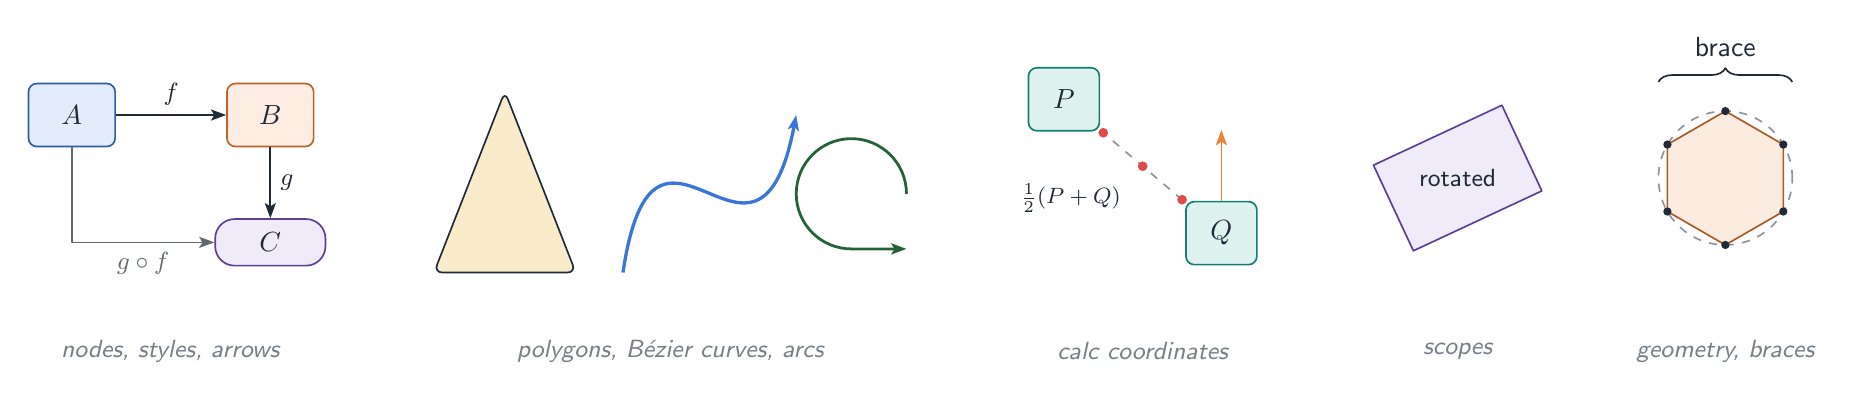
\begin{tikzpicture}[color=Ink, execute at begin picture={\sffamily}, line width=0.6pt, >={Stealth[length=5.5pt, width=4pt, inset=1.2pt]}, line join=round]
  \node[block, minimum width=1.1cm] (n1) at (0,0.6) {$A$};
  \node[block=Orange, minimum width=1.1cm, right=1.4cm of n1] (n2) {$B$};
  \node[pill, below=0.9cm of n2] (n3) {$C$};
  \draw[->] (n1) -- node[pos=0.5, auto, font=\small] {$f$} (n2);
  \draw[->] (n2) -- node[pos=0.5, auto, font=\small] {$g$} (n3);
  \draw[->, color=Ink!70] (n1) |- node[pos=0.75, auto, swap, font=\small] {$g\circ f$} (n3);
  \node[font=\small\itshape, text=Ink!60] at (1.25,-2.4) {nodes, styles, arrows};
  \draw[fill=Yellow!25, rounded corners=3pt] (4.6,-1.4) -- (5.5,0.9) -- (6.4,-1.4) -- cycle;
  \draw[->, color=Blue, line width=1.2pt] (7,-1.4) .. controls (7.4,1.3) and (8.7,-2) .. (9.2,0.6);
  \draw[->, color=Green!60!black, line width=1pt] (10.6,-0.4)
      arc[start angle=0, end angle=270, radius=0.7cm] -- ++(0.7,0);
  \node[font=\small\itshape, text=Ink!60] at (7.6,-2.4) {polygons, Bézier curves, arcs};
  \node[block=Teal, minimum width=0.9cm] (n4) at (12.6,0.8) {$P$};
  \node[block=Teal, minimum width=0.9cm] (n5) at (14.6,-0.9) {$Q$};
  \draw[dashed, color=Ink!50] (n4) -- (n5);
  \node[dot, fill=Red, minimum size=3.5pt] at ($(n4)!0.25!(n5)$) {};
  \node[dot, fill=Red, minimum size=3.5pt] at ($(n4)!0.5!(n5)$) {};
  \node[dot, fill=Red, minimum size=3.5pt] at ($(n4)!0.75!(n5)$) {};
  \node[anchor=north east, font=\footnotesize] at ($($(n4)!0.5!(n5)$)+(-0.15,-0.1)$) {$\tfrac12(P+Q)$};
  \draw[->, color=Orange] (n5.north) -- ($(n5.north)+(0,0.9)$);
  \node[font=\small\itshape, text=Ink!60] at (13.6,-2.4) {calc coordinates};
  \begin{scope}[shift={(17.6,-0.2)}, rotate=25]
    \draw[fill=Purple!12, draw=Purple!70!black] (-0.9,-0.6) rectangle (0.9,0.6);
    \node[font=\small] {rotated};
  \end{scope}
  \node[font=\small\itshape, text=Ink!60] at (17.6,-2.4) {scopes};
  \draw[fill=Orange!15, draw=Orange!70!black] (21,0.65) -- (20.2639,0.225) -- (20.2639,-0.625) --
      (21,-1.05) -- (21.7361,-0.625) -- (21.7361,0.225) -- cycle;
  \draw[dashed, color=Ink!50] (21,-0.2) circle[radius=0.85cm];
  \node[dot, minimum size=3pt] at (21,0.65) {};
  \node[dot, minimum size=3pt] at (20.2639,0.225) {};
  \node[dot, minimum size=3pt] at (20.2639,-0.625) {};
  \node[dot, minimum size=3pt] at (21,-1.05) {};
  \node[dot, minimum size=3pt] at (21.7361,-0.625) {};
  \node[dot, minimum size=3pt] at (21.7361,0.225) {};
  \draw[decorate, decoration={brace, amplitude=5pt, raise=2pt}] (20.15,0.95) -- (21.85,0.95)
      node[midway, auto, outer sep=8pt] {brace};
  \node[font=\small\itshape, text=Ink!60] at (21,-2.4) {geometry, braces};
\end{tikzpicture}
\end{document}
